\documentclass[runningheads]{llncs}
\usepackage[utf8]{inputenc}

\usepackage{graphicx}
\usepackage{amsmath}
\usepackage{amssymb}
\usepackage{arydshln}
\usepackage{xcolor,ulem}

\usepackage{wrapfig}

% Used for displaying a sample figure. If possible, figure files should
% be included in EPS format.
%
% If you use the hyperref package, please uncomment the following line
% to display URLs in blue roman font according to Springer's eBook style:
% \renewcommand\UrlFont{\color{blue}\rmfamily}

\setlength{\parskip}{0cm}
\setlength{\parindent}{1em}

\newcommand{\reals}{\mathbb{R}}

\newcommand{\comment}[3]{{\color{#1} {\bf #2 :} #3}}
%\newcommand{\comment}[3]{}  % suppress comments
% Use these macros to make comments.
\newcommand{\kui}[1]{\comment{blue}{Kui}{#1}}
\newcommand{\yoav}[1]{\comment{purple}{Yoav}{#1}}
\renewcommand{\beth}[1]{\comment{red}{Beth}{#1}}
\newcommand{\david}[1]{\comment{cyan}{David}{#1}}
\newcommand{\zhongkai}[1]{\comment{brown}{Zhongkai}{#1}}

\renewcommand\floatpagefraction{.99}
\renewcommand\topfraction{.99}
\renewcommand\bottomfraction{.99}
\renewcommand\textfraction{.1}   
\setcounter{totalnumber}{50}
\setcounter{topnumber}{50}
\setcounter{bottomnumber}{50}
\setlength{\abovecaptionskip}{0pt}
\setlength{\belowcaptionskip}{0pt}

\title{Towards explainable computer assisted Neuroanatomy}
\author{Kui Qian, Zhongkai Wu, Beth Friedman, David Kleinfeld, Yoav Freund}
\date{May 2022}

\begin{document}

\maketitle

\begin{abstract}
  A fundamental goal of neuroanatomy is the annotation of cells and
  structures.  Manual annotation of structures is based on the spatial
  distribution of cell shape, size, orientation and density.  New
  technology rapid imaging of entire brains at high resolution.
  However, manual identification of structures in these massive
  datasets is prohibitively time consuming.  We present a machine
  learning methodology for developing digital assistants that
  significantly reduce the labor of the anatomist while improving the
  consistency of the annotation.

  Our methodology is based on designing, for each annotation problem,
  a large number of features and using boosting on manually annotated
  images to select the most predictive features.

  We describe two annotation tasks to which we applied this approach.
  The first, more complex task is detecting specific structures in the
  brainstem of the mouse. The second is the detection of individual cells marked
  by a fluorescent dye. We provide the details of both of these
  applications and show that they significantly reduce the anatomist's
  labor in completing these tasks.
  
  %We translate each cell image into a feature vector that
  %includes aspect ratio, orientation and area, as well as additional
  %features derived using a graph Laplacian. The algorithm uses the
  %statistical distribution of these features vectors to identify brain
  %structures.
\end{abstract}

\section{Main}
\subsection{Summary}
We propose a system for detecting anatomical structures in the mouse
brain. Our system takes as input high-resolution images of aligned
sections. It produces as output the estimated center of mass (COM) for
each structure. Each detection is assigned a confidence. High
confidence structures are associated with a visual explanation.

\subsubsection {Significance for Neuroanatomy}
~\\ ~\\
{\bf David and Beth, please expand on the following bullets:}
\begin{itemize}
\item What is Neuroanatomy?
  \item Why is Neuroanatomy important (in the context of the great
    advancements in imaging and recording technology)
\item Why is Neuroanatomy hard? (requires a lot of training, the
  number of trained neuroanatomist is small.)
\item An estimate of the amount of manual labor required to achieve
  common tasks.
\end{itemize}

% Manual neuroanatomical analysis of brain sections is critical for
% creating accurate quantitative results. On the other hand, performing
% neuroanatomical analysis is expensive as it requires many hours of
% work of an expert anatomist.

We consider two labor intensive tasks. Localizing anatomical structure
and counting marked cells. Both tasks involve identifying and marking
locations in images and both require expertise.

A rather obvious but important observation is that while a typical
section will contain hard to identify locations, most of the locations
are easy, in the sense that a person with lesser traing can identify
them reliably.

This observation leads to the following approach to automation. We
use so-called {\em confidence rated detectors}. These detectors
associate with each detection a confidence score. A high confidence
score implies that the example is ``easy''  while the rest are
``hard''. This reduces the workload on the anatomist to the following
tasks:
\begin{itemize}
  \item {\bf Confirming the confident detections} In this step the
    anatomist recieves a small sample of the confident detections and
    verifies that they are correct. The sample size depends on the
    desired accuracy.
    \item {\bf classifiying the unconfident detections} In this step
      the anatomist labels {\em all} of the low confident predictions.
    \item {\bf searching for misses:} In this step the anatomist looks
      for locations that were completely missed by te detector.
  \end{itemize}

{\bf Old itemized list}\\
\begin{itemize}
\item Importance and History
\item Manual detection of brain structures has two major drawbacks, the first is the amount of time needed by an anatomist. The second is inconsistencies between anatomists. Automatic detection has the potential of reducing the time and improving the consistency for this task.
\item Challenges: Variability of images
    \begin{itemize}
        \item biology: animal to animal, gender, generally alien across species, transgenic (differentions to genome due to gene expression)
        \item technical: staining, sectioning (mechanical, optical)
    \end{itemize}
  \end{itemize}
  
\subsubsection{Assistive AI} The traditional vision for AI is to design
an algorithm which can perform as well as, and hopefully better than
an expert human. The explosive growth in machine-learning based AI is
evidence that this vision is becoming a reality.

Indeed, in some domains, such as the game of go \cite{} deep neural
networks (DNN)  have achieved super-human capabilities. In addition,
on highly curated image classification datasets such as ImageNet~\cite{} and
CIFAR~\cite{} DNNs give performance that, some argue, is better than
human. However, there are some significant issues with the application
of DNN to real-world problems 

However, performance on many real world problems the performance of learning algorithms is significantly worse that that of an expert human. There are several reasons for that:
\begin{enumerate}
    \item {\bf Scarcity of training labels} Machine Learning algorithms can be roughly divided into supervised and unsupervised learning. Supervised learning algorithms typically require labeled examples, which, in turn, require large amounts of expert manual labels. Manual labeling by experts is often the limiting factor on the accuracy of the learned model.
    \item {\bf Inter-person and intra-person disagreement}
    The scarcity problem is compounded by the the fact that different people, given the same example, will generate different labels. Moreover, even the same person will give different labels at different times. 
    \item {\bf Training and Test data come from different distributions} Most learning algorithms make the assumption that the training set and the test set are drawn IID~\footnote{Data is IID (Identically and Independently Distributed) if it can be modeled as independent draws from a fixed distribution.}. However, real-world data is typically an agglomeration of different distributions. brain to brain variation is much larger than 
    within brain variation. 
\end{enumerate}

Our system is based on a combination of diffusion maps~\cite{} and Adaboost~\cite{}. We address each of the three problems above in turn.

\subsubsection{Old stuff}
In order to create robust classifiers, that do not need
to be retrained on each brain, we need a learning algorithm that
identifies robust patterns that are preserved across brains.
identifies patterns that are consistent across significant variations
in the images.  The development of learning algorithms that are robust
with respect to the nuisance variations from brain to brain.

A second issue that is the variability between labelers. In other
words, different experts, working independently, sometimes provide
different labels. This is especially the case when annotating the
boundary of a structure.  Data regarding such variability is not easy
to come by because it requires that several anatomists independently
annotate the same images.  Significant disagreement levels are well
known in medical diagnostics and are studied under the title
``inter-rater variability''~\cite{gellhorn2013inter}. As can be
expected, the level of disagreement varies from structure to structure
and from cell to cell. Some structures are easy to identify and have
high inter-rater agreement. Other are hard and can result in
disagreements that remain even the different raters discuss the case.

A disagreement on the correct annotation of a specific structure or
cell puts in question the notion of a ``ground truth'', and,
consequently, the accuracy of a classifier.






``easy'' and result in annotations that are very similar, while others
are ``hard'' and result in highly varying annotations.

Our system is based on the distinction between easy and hard
instances. With each detection it associates a numeric measure of
``confidence''.


in the labeling between different anatomists. When the variation
between anatomist is large the meaning of ``better than human''
becomes less clear.


black-box approaches to computer vision
are often sensitive to small changes in the way images are acquired.

In the context of section based neuroanatomy such changes include
variability in staining, sectioning and slicing.
vary.

\subsubsection{Cell based approach}  Most CNN-based method of image
analysis are based on the concept of a sliding window. This implies
that an
y explanation provided by the CNN is based on the content of one or more windows. Windows need to be large enough to capture the image statistics. This means that a typical window contains 10-100 cells.
On the other hand, anatomist base their analysis on cytoarchitecture, which, in turn, is based on the shapes of individual cells and the relationshp between them. This makes it harder for the anatomist to understand the decisions of the detector.
\begin{wrapfigure}{R}{0.65\textwidth}
  \centering
  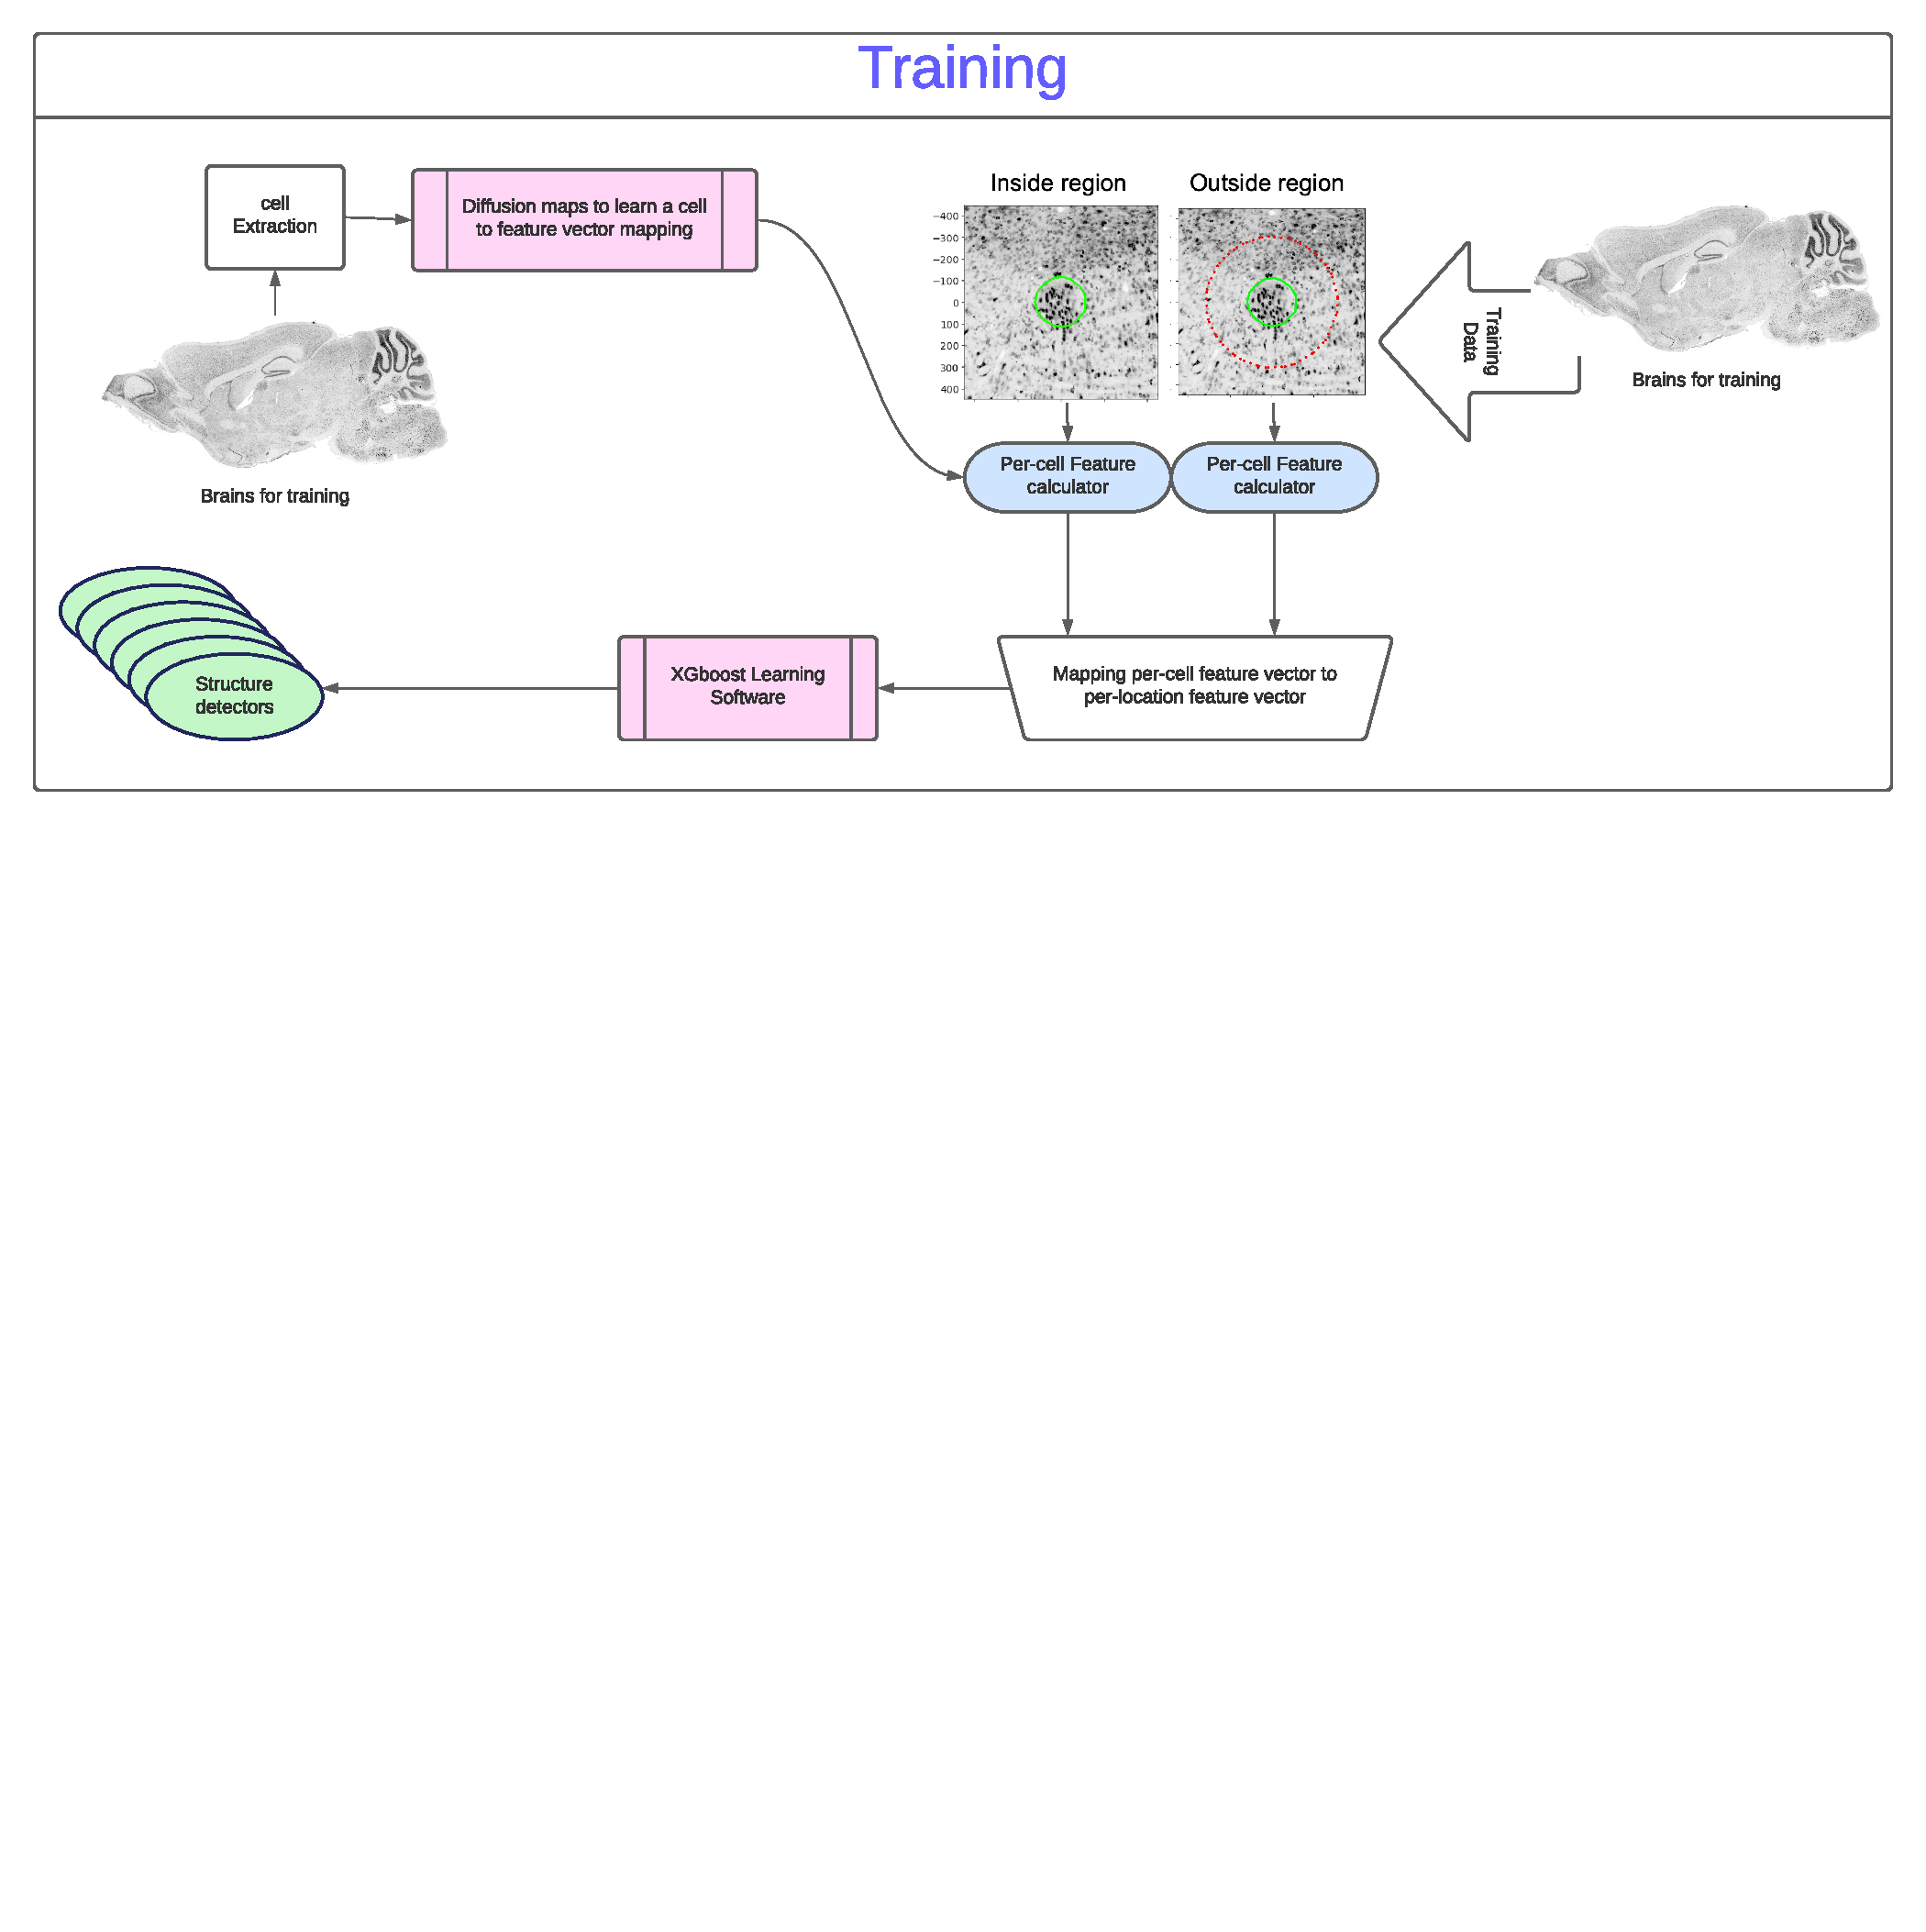
\includegraphics[width=0.6\textwidth]{figures/Training.pdf}
  \caption{Training \label{fig:training}}
\end{wrapfigure}

To remedy this problem and make the detections explainable, we use individual cells as our basic unit. 

The overall design of the system is shown in Figure xxx. The system can be partitioned into two parts. The training algorithm and the trained detector.

\subsection{System Inputs}
To train the detectors we combine three sources of information:
\begin{itemize}
    \item {\bf Images of aligned sections:} The Nissl images of XX brains are the primary information source. They are also by far the largest at XXX GB per brain.
    \item {\bf The Atlas} is a representation of the shape of each structure and the relative locations of the structures. The atlas was constructed through a concensus ....
    \item {\bf COMs for individual brains:} For XX brains we had an anatomist locate the COM ....
\end{itemize}

\subsection{System components}

\begin{enumerate}
\item{\bf Cell extraction and shape parametrization}
An image of a single cell is typically around 50$\times$50 pixels, or a 2500 dimensional vector. The dimension of this representation is too high for effective machine learning. We therefor seek a dimensionality reduction mapping. This mapping consists of three parts:
\begin{enumerate}
    \item {\bf Normalization:} We normalize the image of the cell in three ways. We 
    shift the grey-levels so that the mean is XXX, scale the grey levels so that the standard deviation is YYY, and rotate the image so that the long axis of the cell is in angle zero. The three parameters associated with the normalizations define three features.
    \item {\bf Standard shape features}: we use the Hu features: x,y,z...
    \item{ \bf  Diffusion maps}: Diffusion Mapping~\cite{Belkin,
        Coifman} is a non-linear dimensionality reduction method that
      is based on a graphical representation of the data and on the
      Laplace operator on graphs.
      \end{enumerate}
\end{enumerate}
      \subsubsection{ Characterizing Cytoarchitecture} uses Difference between the CDFs for inside and outside of each structure (based on manually annotated structure boundaries). 
\subsubsection { Structure detectors} Combine the difference-of-CDF
features using boosted trees (XGBoost). Each structure has a
corresponding detector.

\subsubsection { Structure detection confidence} The confidence of structure
  detections is measured by the prediction margin and by the sharpness
  of the detection peak.
\begin{wrapfigure}{R}{0.65\textwidth}
\centering
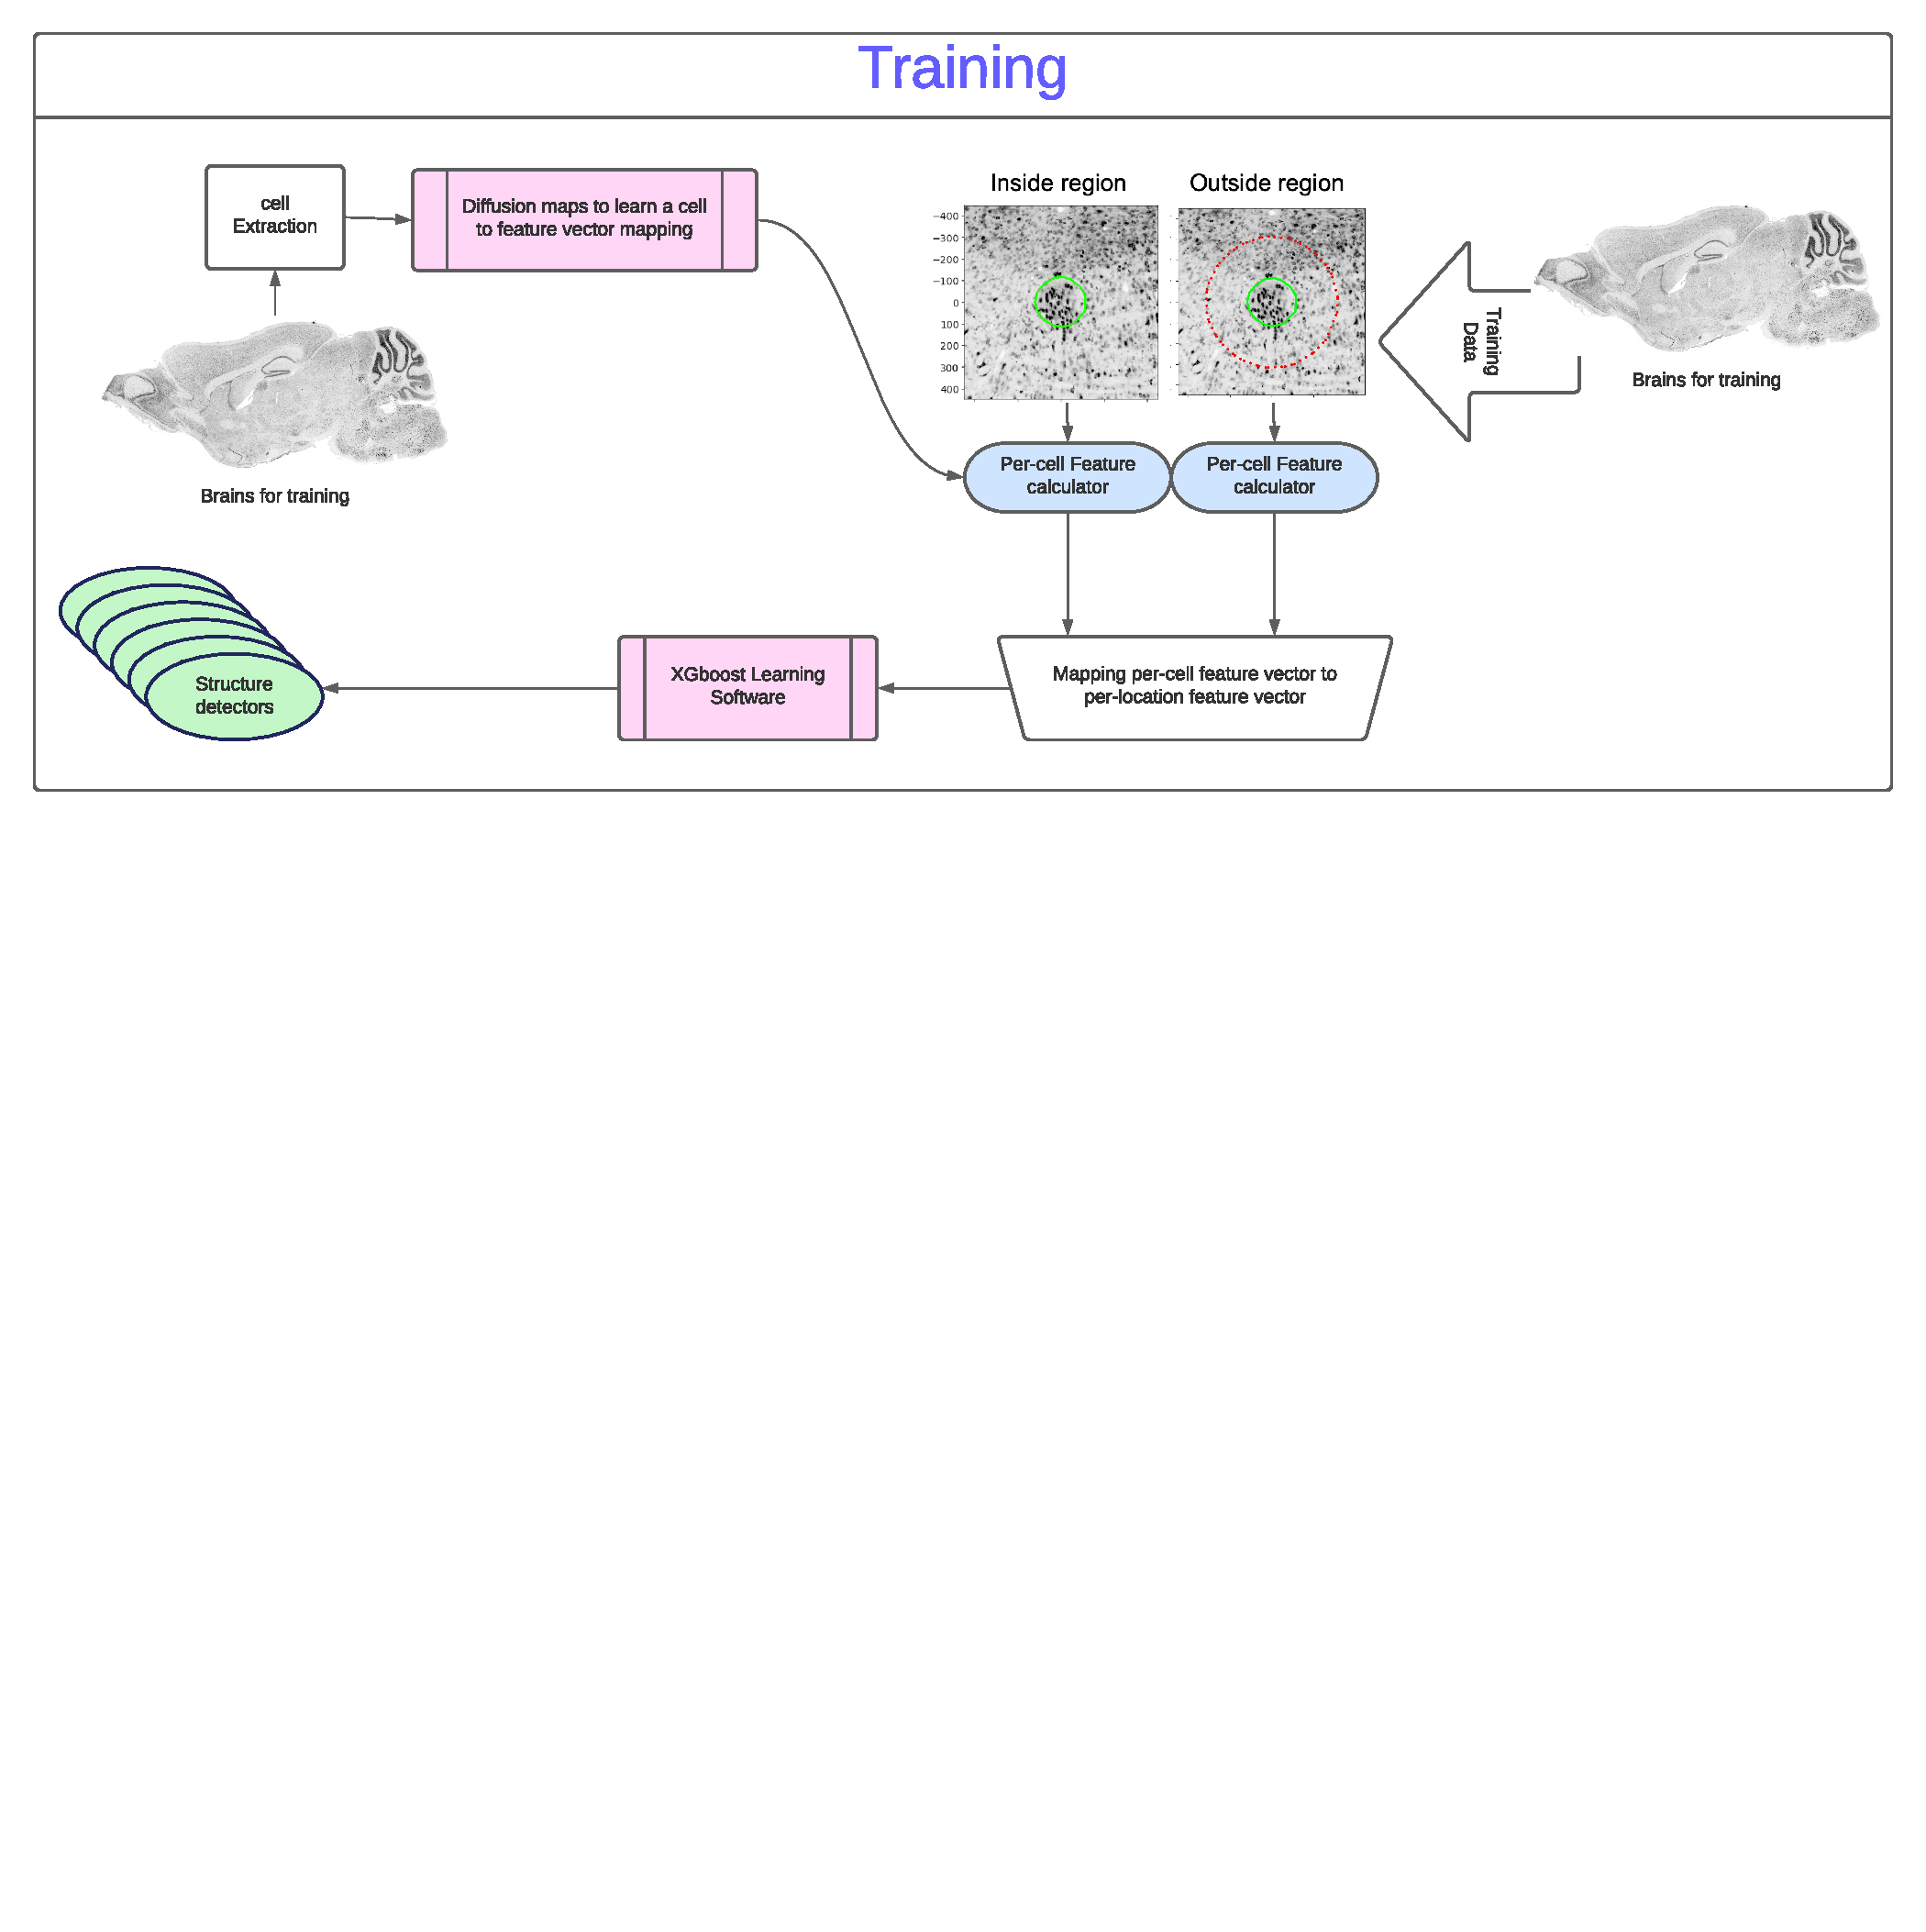
\includegraphics[width=0.6\textwidth]{figures/Training.pdf}
\caption{Training \label{fig:training}}
\end{wrapfigure}
y
\subsubsection { Structure detection explanation}

\iffalse
which is based on cells as the basic unit. Doing so provides an explanation for the detector's decision. We use unsupervised learning to find a dimensionality reducing mapping for cell shapes. We make efficient use of manual annotations by estimating the shape of each structure from a few brains and anatomists. We leverage this information in the detector training by having the anatomist identify the location of the center of mass for each structure.
\fi
\section{Results}

\begin{itemize}
    \item Detection results, with confidence levels, consistency with Beth.
    \yoav{A lot of stuff here. Detection accuracy and confidence table, full table will probably go in the appendix, the figure of improvement. Relationship between beth, rough alignment and detection.}
    \item {\bf Explaining detections} The explanation of the detection is expressed in terms of cells whose shape gives evidence to the structure.
    \yoav{Put here an image consisting of 2/3 detection explanations to show the explanation power. Specifically, there is a structure we detect well even though in different brains the contrast and brightness are very different}
\item {\bf Cell shape parametrization} Uses a combination of Hu moments and dimensionality reduction using eigen-maps.
\begin{itemize}
    \item Eigen-maps learn a dimensionality reducing mapping cell shape to a ten dimensional representation.
    As it is an unsupervised method it requires no human labeling. We take advantage of the very large number of cells in single brain. 
    \item Each brain creates a different mapping, however, the mappings can be made consistent by adding a linear transformation. This creates a stable parametrization and makes the detections more consistent.\yoav{scatter-plots of cell images. after transformation. Figure explaining transformation.}
\end{itemize}

\end{itemize}

\section{Detecting marked cells}

William to put the {\em latest} table here. and write a detailed
explanation of the table.

To discuss:
\begin{itemize}
\item The amount of manual work that it takes to manually mark cells.
\item inter-rater and intra-rater disagreement rate.
\item How to count false detections "with approximately correct
  detections detection".
\item How to quantify reduced mental load of QA vs detection.
\end{itemize}


\section{Methods}
In this section we provide more details on the algorithms we use in
our system. The full code is available from github...

\begin{itemize}
\item Cell based features.
\item Diffusion mapping.
\item Calibration of the diffusion features.
\item Region features and CDFs.
\item Boosting and XGBoost.
\item Localizing structures. Rough alignment, computing detections
  scores, computing autocorrelation and asigning confidence.
\item Using the system for brain-to-atlas alignment.
\item Generating explanations.
\end{itemize}

\section{Unplaced figures}

\begin{figure}[t]
  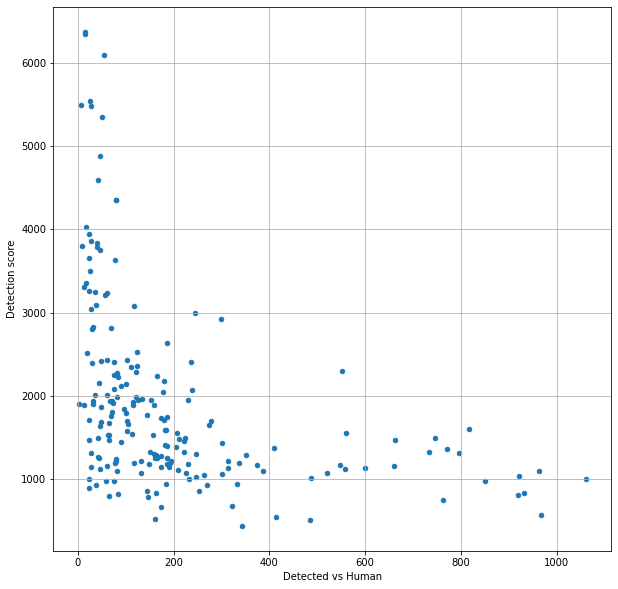
\includegraphics[width=\textwidth]{figures/DetectionConfidenceVsError.png}
  \caption{}
\end{figure}

\begin{figure}[t]
  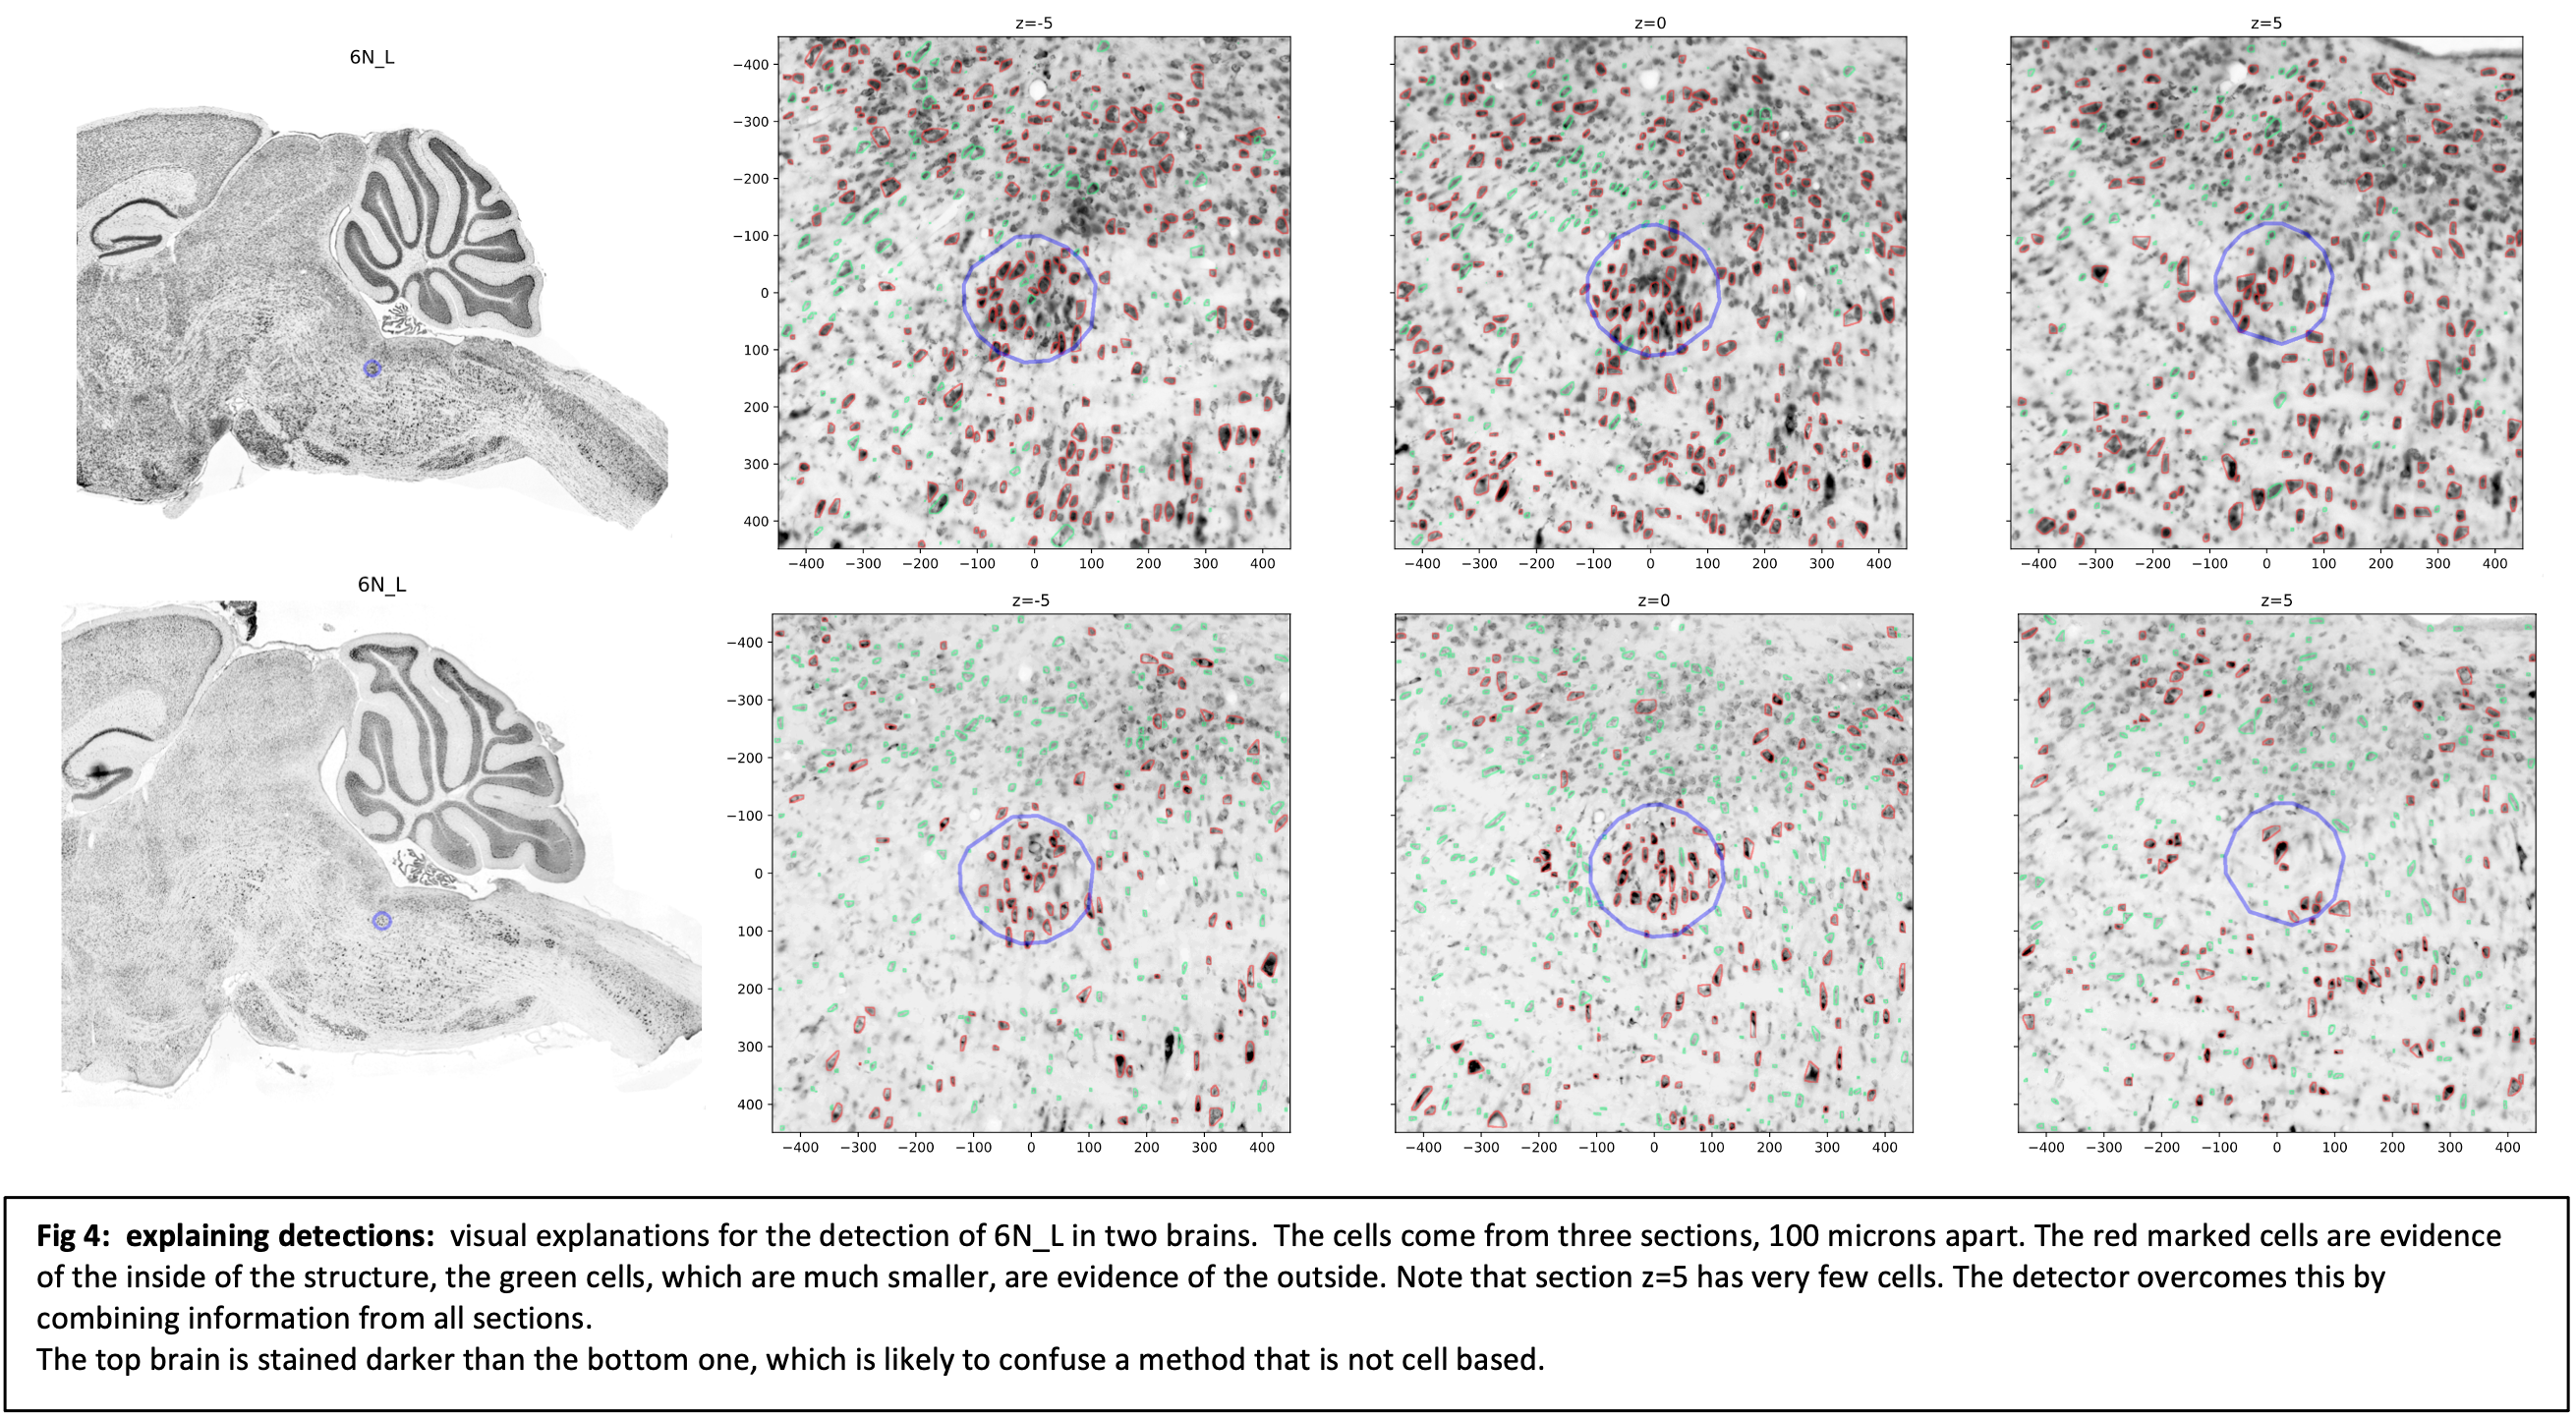
\includegraphics[width=\textwidth]{figures/DetectionsExplanations.png}
  \caption{}
\end{figure}

\begin{figure}[t]
  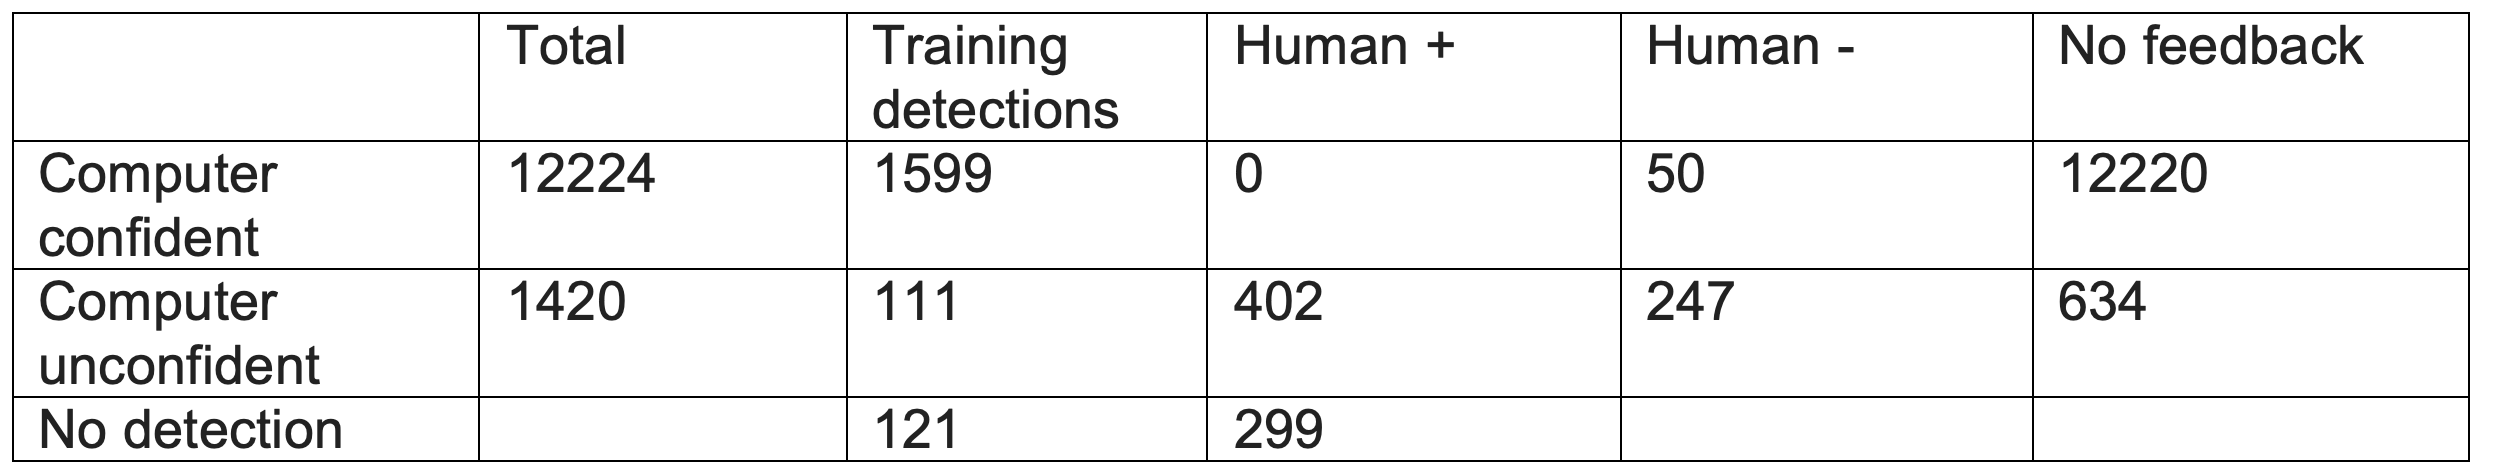
\includegraphics[width=\textwidth]{figures/MarkedCellsDetectionNumbers.png}
  \caption{}
\end{figure}

\begin{figure}[t]
  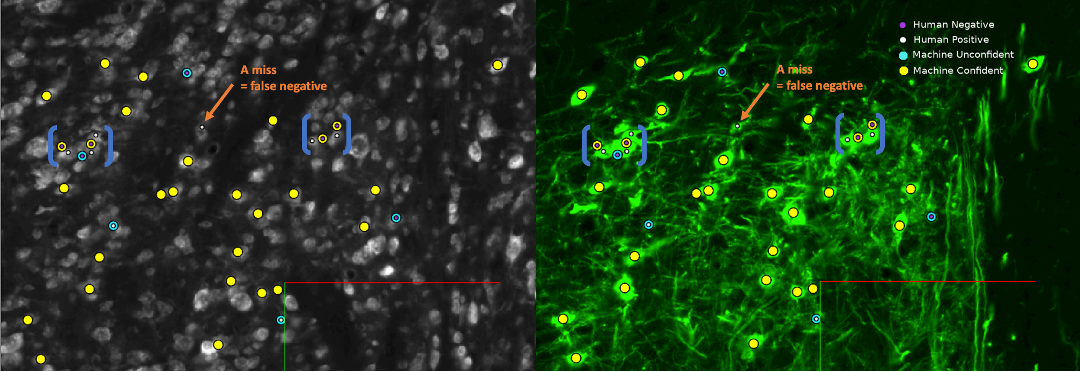
\includegraphics[width=\textwidth]{figures/Marked_cell_detections.png}
  \caption{}
\end{figure}

\begin{figure}[t]
  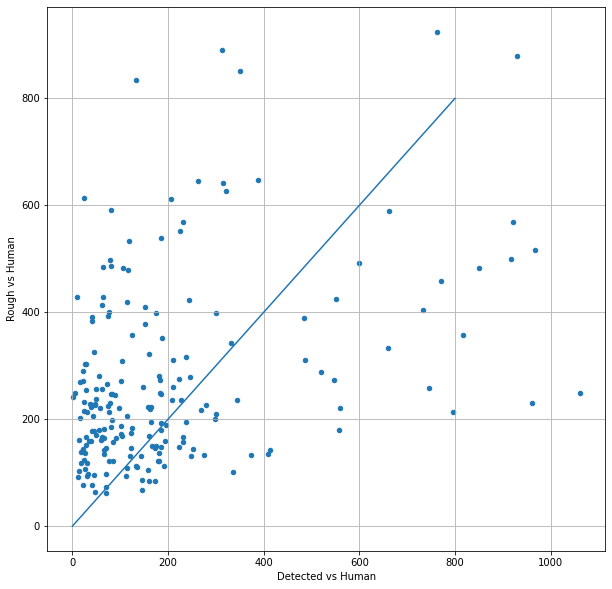
\includegraphics[width=\textwidth]{figures/RoughVSDEtection.png}
  \caption{}
\end{figure}

\begin{figure}[t]
  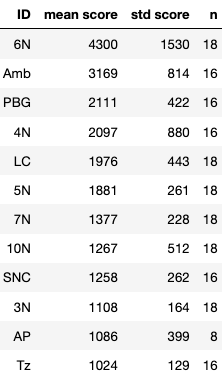
\includegraphics[width=\textwidth]{figures/ScoresOfStructures.png}
  \caption{}
\end{figure}

\end{document}


